\chapter{Electromagnetic induction}

\section{Soft iron ring}
\begin{problem}
A soft iron ring of variable cross-section has two coils wound around it.
One coil has seven turns. The other, of three turns, is connected to a
d.c. supply. Distinguish the quantities \term{magnetic field},
\term{magnetic flux}, \term{magnetic flux density} and \term{magnetic flux linkage}---which
quantity is the same inside each coil?
\end{problem}

\begin{itemize}
	\item \term{Magnetic flux density} \(B\) is related to how tightly packed the magnetic field lines
	      are within a material.
	\item \term{Magnetic flux} \(\Phi_B\) concerns the number of magnetic field lines \it{in total} across
	      a certain surface area.
	\item \term{Magnetic flux linkage} \(\Phi\) accounts for the fact that magnetic flux passes through
	      each turn in a coil. It is, therefore, related to the number of turns in the coil.
	\item What \term{magnetic field} means here is unclear, but it must be related to its strength, magnetic flux
	      density.
\end{itemize}

Eliminate magnetic flux density because a current passes through only one of the coils (but not the other);
eliminate magnetic flux linkage because the number of turns in each coil differ;
eliminate magnetic field because it is somehow related to magnetic flux density (and cannot be an option).

The \hil{magnetic flux} through both coils is the same. The total number of magnetic field lines
across the whole system doesn't change since there aren't any changing quantities.


\section{Copper rod}
\begin{marginfigure}
	\begin{tikzpicture}
		\draw[pattern={Dots[distance=1em, radius=1.5pt]}, pattern color=black!50] (0, 0) rectangle (6, 4);
		\draw[very thick, color=black] (0.5, 2.75) -- (6, 2.75);
		\node[above right] (A) at (0.5, 2.75) {\(A\)};
		\draw[very thick, color=black] (0.5, 2.75) -- (6, 1);
		\draw[pattern=north west lines, pattern color=jiyopink, draw=jiyopink, very thick] (4, 3) rectangle (4.15, 1.25);
		\node[above right] (C) at (4.15, 2.75) {\(C\)};
		\node[below right] (B) at (4.15, 1.5) {\(B\)};
		\draw[-Stealth, very thick] (4.15, 2) -- (4.8, 2) node[right] {\(\va{v}\)};
		\node[above right] (T) at (0, 0) {\(\va{B}\) (out of paper)};
	\end{tikzpicture}
	\caption{Sliding copper rod}
	\label{fig:sliding-rod}
\end{marginfigure}
\begin{problem}
\Cref{fig:sliding-rod}. A copper rod is sliding on two conducting rails which make an angle of \(\theta = \qty{15}{\degree}\)
to each other. The rod moves to the right with a constant speed \(v = \qty{0.50}{\metre\per\second}\).
A uniform magnetic field \(B = \qty{0.30}{\tesla}\) is applied perpendicularly out of the plane
of the paper.

What is the magnitude of the average emf induced in the triangle \(ABC\) in a period of
\(\Delta t = \qty{10}{\second}\) after the rod passes point \(A\)?
\label{prob:2i}
\end{problem}

Over \(\qty{10}{\second}\), the rod covers the area of the triangle \(ABC\).
This area \(A = \f{1}{2}\ab|AC|\ab|BC|\).
\begin{align*}
	A & = \f{1}{2}\ab|AC|\ab|BC|                      \\
	  & = \f{1}{2}\ab|AC|\times\ab|AC|\tan\theta      \\
	  & = \f{1}{2}v\Delta t\times v\Delta t\tan\theta \\
	  & = \f{1}{2}v^2{\ab(\Delta t)}^2\tan\theta
\end{align*}

The total change in magnetic flux is then \(\Delta\Phi = B\Delta A\).
\begin{equation*}
	\Delta\Phi = \f{1}{2}Bv^2{\ab(\Delta t)}^2\tan\theta
\end{equation*}

Then the average emf will be the total change in magnetic flux \(\Delta\Phi\)
over the total time taken \(\Delta t\).
\begin{align*}
	\left\langle\varepsilon\right\rangle & = \ab|\f{\Delta\Phi}{\Delta t}|                  \\
	                                     & = \f{Bv^2{\ab(\Delta t)}^2\tan\theta}{2\Delta t} \\
	                                     & = \f{1}{2}Bv^2\ab(\Delta t)\tan\theta            \\
	                                     & = \hil{\qty{0.100}{\volt}}
\end{align*}

\begin{problem}
What is the instantaneous emf at any time \(t\)
after the rod has passed point \(A\)?
\label{prob:2ii}
\end{problem}
We figured out previously that the area covered is a function of time,
while magnetic flux density is a constant.
\begin{equation*}
	A\ab(t) = \f{1}{2}v^2t^2\tan\theta
\end{equation*}
Since induced emf \(\varepsilon = \odv{\Phi}{t}\), then we can say that
\begin{align*}
	\varepsilon & = \odv{\Phi}{t}                                 \\
	            & = B\odv{A}{t}                                   \\
	            & = B\times\odv{}{t}\ab(\f{1}{2}v^2t^2\tan\theta) \\
	            & = Bv^2t\tan\theta
\end{align*}

\begin{problem}
If we average the instantaneous emf (\cref{prob:2ii}) over the same \(\qty{10}{\second}\),
will we arrive at the same answer as in \cref{prob:2i}?
\end{problem}
From \cref{prob:2ii}, the \it{average} emf is
\begin{align*}
	\left\langle\varepsilon\right\rangle & = \f{Bv^2t\tan\theta}{t} \\
	                                     & = Bv^2\tan\theta
\end{align*}
Our answer in \cref{prob:2i} is \(\left\langle\varepsilon\right\rangle = \f{1}{2}Bv^2t\tan\theta\),
which still includes a factor of \(t\). This is because the \it{instantaneous} emf in \cref{prob:2ii}
does not account for the emf accumulated throughout the whole \(\qty{10}{\second}\) journey.


\section{Falling magnet}
\begin{problem}
A short bar magnet is dropped vertically downwards into a copper pipe.
It takes longer than `usual' for this magnet to emerge at the bottom.
Why does the magnet fall so slowly?
\end{problem}
Assume the magnet falls south pole first.

\subsection{Qualitative analysis}
From the viewpoint of the top of the pipe,
\begin{itemize}
	\item There is a decreasing upward magnetic flux\sidenote{Within the magnet, the magnetic flux flows from South to North! It flows from North to South \it{outside} the magnet.} as the magnet falls downwards.
	\item The induced current in the pipe must induce an upward magnetic field to oppose the flux change.
	\item The induced current in the pipe runs anti-clockwise to the observer (and clockwise to the magnet), which forms a North pole facing downward towards the magnet's North pole.
	\item There is an attractive force pushing the magnet upward.
\end{itemize}

From the viewpoint of the bottom of the pipe,
\begin{itemize}
	\item There is an increasing upward magnetic flux as the magnet falls downwards.
	\item The induced current in the pipe must induce a downward magnetic field to oppose the flux change.
	\item The induced current in the pipe runs clockwise, which forms a South pole facing upward towards the magnet's South pole.
	\item There is a repulsive force pushing the magnet upward.
\end{itemize}

Both these forces push the magnet upward, opposing the gravitational force of the magnet pulling it downwards.
The downward acceleration of the magnet is reduced.

\subsection{Quantitative analysis}
Take \(x\) to be the width of the magnet and the width of the pipe\sidenote{This is so that the magnet fits tightly in the pipe!}.
Let \(r\) and \(L\) be the thickness and length of the pipe, and \(\rho\) the resistivity of copper.
We start with \(B_0\) being the magnetic flux density at the top of the pipe, and \(v\) its velocity.

For a period of time \(t = \lf{x}{v}\) after the start of the magnet's fall,
the magnet of width \(x\) falls through a distance of \(x\), covering an area of \(x^2\).\sidenote{The upwards direction is positive.}

\begin{align*}
	\varepsilon = -\odv{\Phi_B}{t} & = -B_0\odv{A}{t}          \\
	                               & = -B_0\f{x^2}{\lf{-x}{v}} \\
	                               & = B_0vx
\end{align*}

The resistance of this short segment of the pipe the magnet falls through is
dependent on the length of the segment \(x\) and the cross-sectional area \(rx\).
\begin{align*}
	R & = \lf{\rho x}{rx} \\
	  & = \lf{\rho}{r}
\end{align*}

The power dissipated in this time is \(P = \lf{\varepsilon^2}{R}\).
\begin{align*}
	P & = \lf{\varepsilon^2}{R}    \\
	  & = \f{{B_0}^2v^2x^2r}{\rho}
\end{align*}

Due to gravity, the magnet loses gravitational potential energy at a rate of \(\odv{U}{t} = mgv\).
Equating the power dissipated (rate of energy loss) and the rate of loss of gravitational potential energy,
\begin{align*}
	mgv & = \f{{B_0}^2rv^2x^2}{\rho} \\
	v   & = \f{mg\rho}{{B_0}^2rx^2}
\end{align*}

Lastly, since the time taken for the magnet's descent \(T = \f{L}{v}\), then
\begin{equation}
	T = \f{{B_0}^2Lrx^2}{mg\rho}
	\label{eq:lenz-time}
\end{equation}
Comparing \cref{eq:lenz-time} to the well-known result \(T' = \sqrt{\lf{2L}{g}}\) under gravity only, \(T > T'\)
for sufficiently large values of \(B_0\) and sufficiently small values of \(\rho\).

\section{Critical damping}
\begin{figure}[htpb]
	\centering
	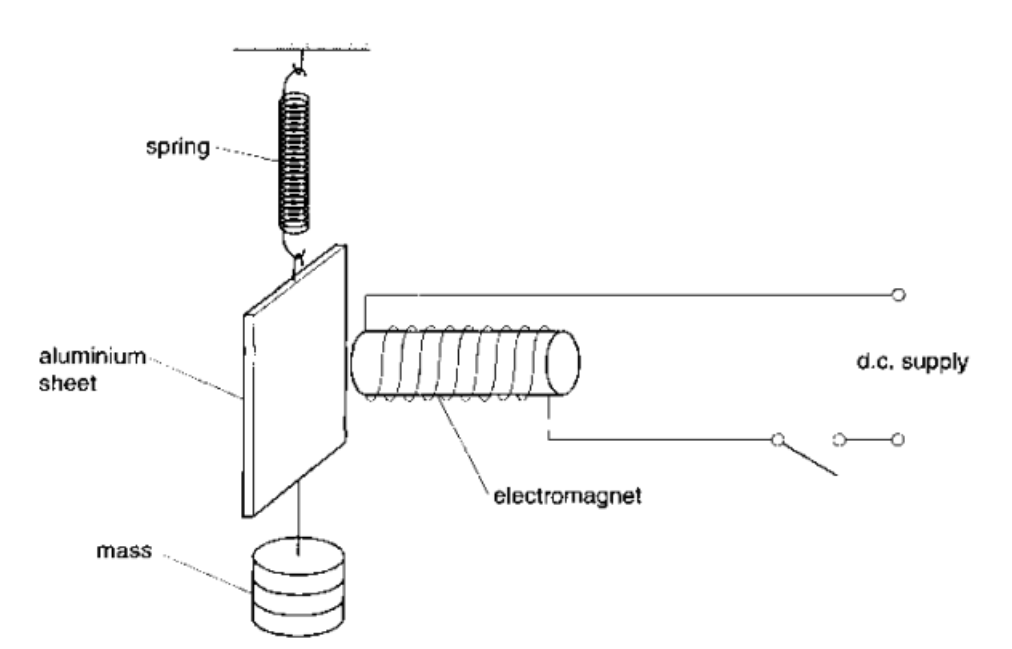
\includegraphics[scale=.5]{assets/spring-aluminium.png}
	\caption{Oscillating system}
	\label{fig:spring-aluminium}
\end{figure}
\begin{problem}
\Cref{fig:spring-aluminium}. A helical spring is clamped vertically.
The free end of the spring is attached to
an aluminium sheet and a mass. An electromagnet is placed near the centre of the
aluminium sheet.

The electromagnet is \bf{off}. The mass is displaced vertically and released.
This procedure is then repeated with the electromagnet \bf{on}.
Sketch the variation of the displacement of the mass \(x\) with time \(t\).
\end{problem}

With the electromagnet \bf{off}, the mass undergoes simple harmonic motion.
Taking the upwards direction as positive, the mass begins with a negative initial displacement.

With the electromagnet \bf{on}, a magnetic field is generated.
As the aluminium sheet oscillates, it experiences a changing magnetic flux, which
induces an emf proportional to the rate of change of magnetic flux. Since the
aluminium sheet contains \it{closed electric paths}, induced \term{eddy currents}
cause Joule heating, which dissipate the sheet's energy.

As the oscillations are continually dampened, their amplitude decreases.
Since the velocity of the sheet also decreases with every oscillation,
the time taken for every oscillation increases.

\begin{center}
	\begin{tikzpicture}
		\begin{axis}[
				% tuftelike,
				width=\textwidth,
				xtick=\empty,
				ytick={-.5, 0, .5},
				yticklabels={\(-x_0\), \(0\), \(x_0\)},
				xlabel=\(t\),
				ylabel=\(x\),
				ymin=-.6,
				ymax=.6,
				xmin=0,
				domain=0:7.27278,
				samples=200,
				axis lines=middle,
			]
			\addplot[jiyopink, ultra thick] {-0.5 * cos(deg(5 * x))};
			\addplot[jiyoblue, ultra thick] {-0.5 * exp(-0.2 * x) * cos(deg(5 * x * exp(-0.02 * x)))};
			\legend{off, on};
		\end{axis}
	\end{tikzpicture}
\end{center}

\section{Non-uniform magnetic field}
\begin{marginfigure}
	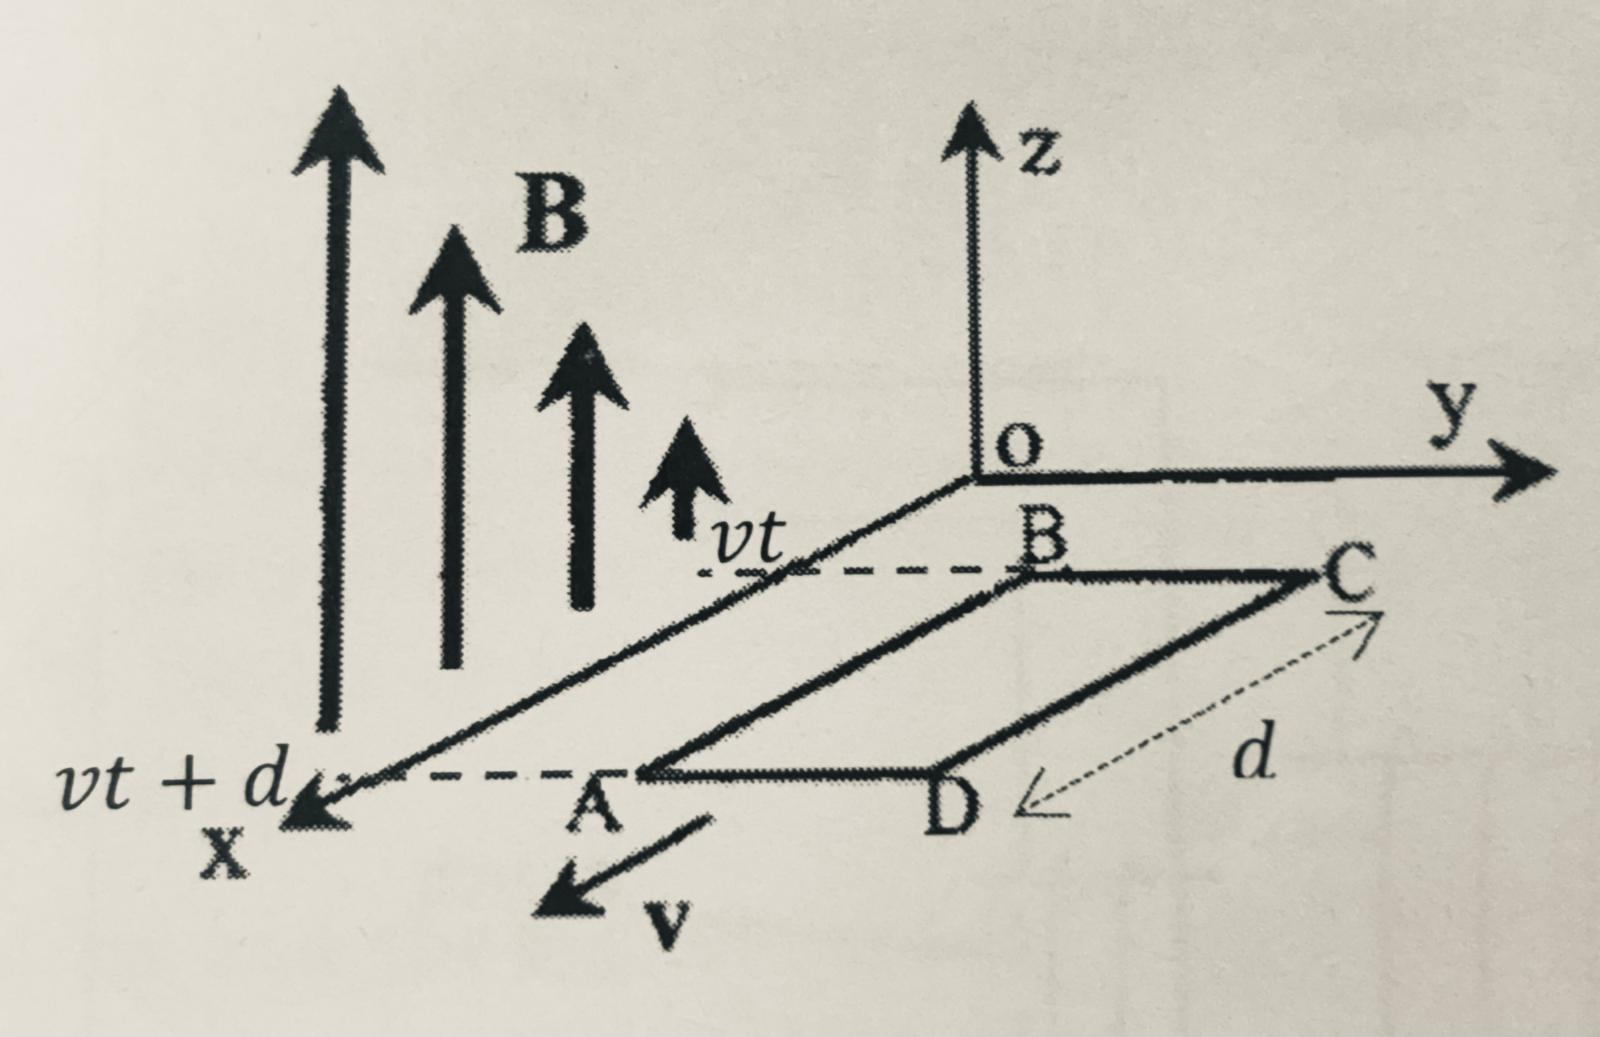
\includegraphics[scale=0.8]{assets/non-uniform-B.jpeg}
	\caption{Non-uniform \(\va{B}\)-field}
	\label{fig:non-uniform-B}
\end{marginfigure}
\begin{problem}
\Cref{fig:non-uniform-B}. Consider a rectangular conducting loop moving with constant speed \(v\)	in a non-uniform
magnetic field. The loop lies in the \(xy\)-plane, while the magnetic field
points in the positive \(z\)-direction, such that its magnitude
varies along the \(x\)-axis, \(\va{B} = B_0x\kk\). When the coil begins moving,
the side \(BC\) is flush against the \(y\)-axis.

Deduce the emf induced in the loop from
\begin{itemize}
	\item an \term{inertial frame of reference}---the observer watches the loop move with constant speed.
	\item a \term{center-of-mass frame of reference}---the observer moves along with the loop.
\end{itemize}
\end{problem}

\subsection{Stationary frame}
After an infinitesimally short period of time \(\odif{t}\), the loop would have moved an
infinitesimally short distance \(\odif{x}\) along the \(x\)-axis.
The change in magnetic flux \(\odif{\Phi_B} = A\odif{B} = Ld\cdot B_0\odif{x}\).

\begin{align*}
	\abs{\varepsilon} & = \ab|\odv{\Phi_B}{t}| \\
	                  & = LdB_0\odv{x}{t}      \\
	                  & = LdB_0v
\end{align*}

\subsection{Moving frame}
An observer moving along with the coil will view that the coil is stationary.
Therefore, there is no longer any magnetic force on the coil, since magnetic force
requires a non-zero velocity (\(F_B = Bqv\)).

On a stationary unit charge, only an electric force \(F_E = qE\) is exerted.
There must be an \it{electric force} in the moving frame!

Using Fleming's left-hand rule, this electric field points in the
positive \(y\)-direction, since the magnetic field lines point in the
positive \(z\)-direction.
Since the magnetic field appears to be `moving' with velocity \(-v\) behind
the coil, we get
\begin{align*}
	E_x & = 0      \\
	E_y & = -B_0vx \\
	E_z & = 0
\end{align*}

We can check how consistent we are by using the Lorentz force law \(\va{F} = q\ab(\va{v}\times\va{B}+\va{E})\).
In the stationary frame,
\begin{align*}
	\va{F} & = q\va{v}\times\va{B}  \\
	       & = qv\ii \times B_0x\kk \\
	       & = -qB_0vx\jj
\end{align*}
And in the moving frame,
\begin{align*}
	\va{F}' & = q\va{E}'        \\
	        & = q\ab(-B_0vx\jj) \\
	        & = -qB_0vx\jj
\end{align*}

\hil{Electric and magnetic fields are not independent objects!}
They are two aspects of a single electromagnetic field instead.

To find the induced emf, we use \(\varepsilon = \oint\va{E}\cdot\odif{\va{l}}\),
where \(\varepsilon\) denotes the work done in pushing a unit charge around
the full loop. This is easy, because we've established before that the electric field
only exists in the \(y\)-direction.

The long sides \(AB\) and \(CD\) don't count, since they aren't along the \(y\)-axis.
The short sides \(AD\) and \(BC\) run in the \(y\)-direction. Establishing the position
of \(BC\) as \(x = x_0\), we can find expressions for the electric fields along both short sides.

Along \(AD\), \(E_y = -B_0vx_0\). Along \(BC\), which is at position \(x = d + x_0\),
\(E_y = -B_0v\ab(d+x_0)\).

Then we integrate to get the work done per unit charge---induced emf:
\begin{align*}
	\varepsilon       & = \oint\va{E}\cdot\odif{\va{l}}           \\
	                  & = L\ab(\eval{E_y}_{BC} - \eval{E_y}_{AD}) \\
	                  & = L\ab[-B_0v\ab(d+x_0) + B_0vx_0]         \\
	                  & = -B_0vLd                                 \\
	\abs{\varepsilon} & = B_0vLd
\end{align*}

\hil{Both the stationary and moving frames of reference yield the same answer!}

\section{Jumping ring}
\begin{problem}
An aluminium ring is fitted around a vertical steel rod connected to an a.c.
supply. A copper coil is connected at the base of the steel rod.
When the supply is turned on, the aluminium ring appears to `jump'
up and down along the steel rod. Why?
\end{problem}
Because the supply is a.c., the magnetic field induced
is constantly changing in magnitude and direction. There is a
changing magnetic flux about the aluminium ring, which induces a
changing emf (Faraday's law) and an induced current flows.

When the current is increasing in the upward direction, an
induced current flows downwards (Lenz's law) to oppose the change in flux linkage.

Similarly, when the current is increasing in the downward direction, an
induced current flows upwards to oppose the change in flux linkage.

\begin{problem}
What happens when the aluminium ring is replaced by a broken ring,
and then by a perforated ring?
\end{problem}
The broken ring can no longer carry an induced current, so it
cannot `jump up'. The perforated ring has a smaller surface
area in which induced current can flow through, so it will `jump up'
to a lower height.
